\section{Poly\-CDI.h File Reference}
\label{PolyCDI_8h}\index{PolyCDI.h@{PolyCDI.h}}
{\tt \#include $<$Base\-CDI.h$>$}\par
{\tt \#include $<$vector$>$}\par
{\tt \#include $<$cstring$>$}\par


This graph shows which files directly or indirectly include this file:\begin{figure}[H]
\begin{center}
\leavevmode
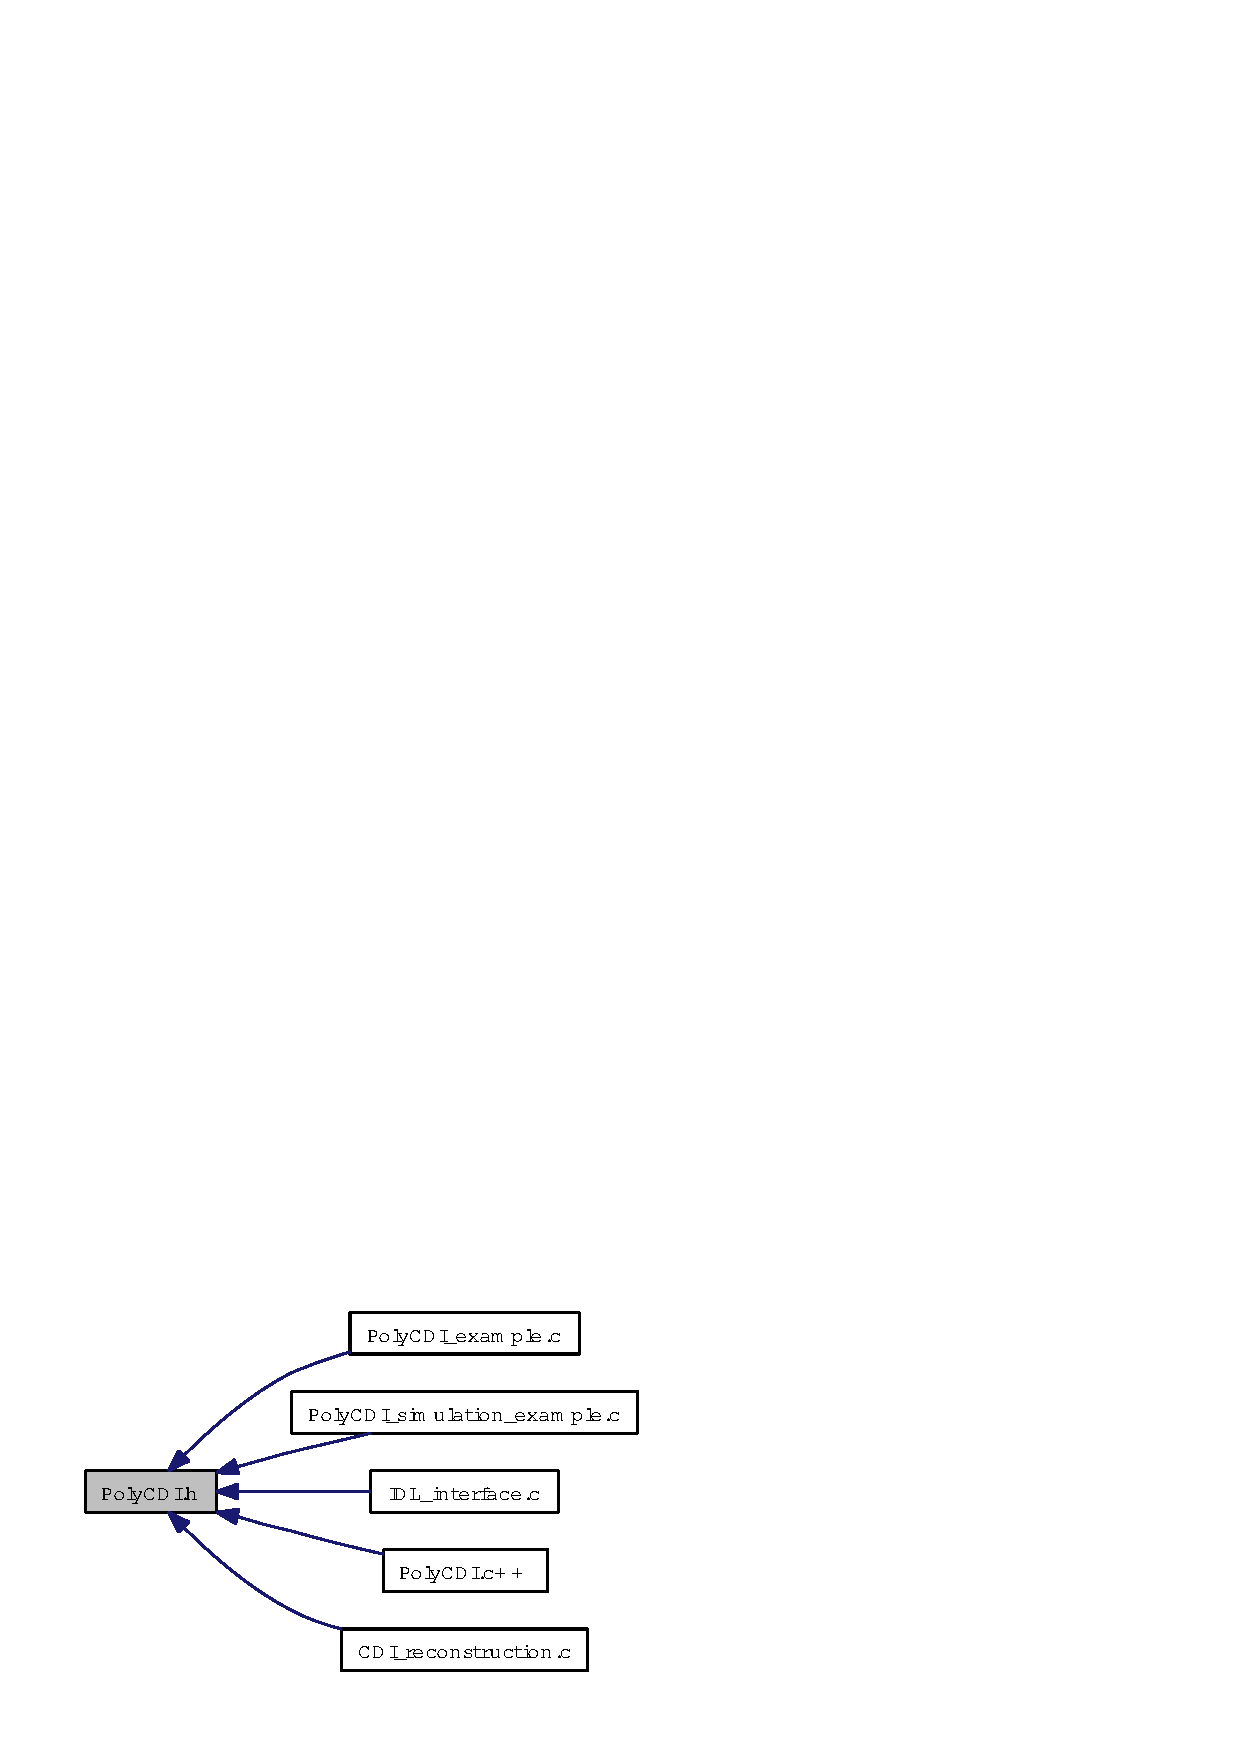
\includegraphics[width=155pt]{PolyCDI_8h__dep__incl}
\end{center}
\end{figure}
\subsection*{Data Structures}
\begin{CompactItemize}
\item 
class \bf{Poly\-CDI}
\begin{CompactList}\small\item\em The class which performs partially coherent reconstruction. \item\end{CompactList}\end{CompactItemize}
\subsection*{Defines}
\begin{CompactItemize}
\item 
\#define \bf{WL}~0\label{PolyCDI_8h_ec70dd1e9ed3c793ea9abbcceff787a4}

\item 
\#define \bf{WEIGHT}~1\label{PolyCDI_8h_b82d5fd8e274d3d125a1e382ceceab7c}

\end{CompactItemize}


\subsection{Detailed Description}


Definition in file \bf{Poly\-CDI.h}.